\def\ascWiki{https://mp-force.ziti.uni-heidelberg.de/asc/doc/wiki/wikis/Technical-notes/ASC-server-hardware}

\chapter{Characterization \& Benchmarks}

  \section{Structured Matrices as Baseline Performance Indicators} \label{sec:test-matrices}

    In order to characterize the C3SR-format's storage scheme two families of matrices derived from structured grids are
    inspected. The matrices correspond to the 3-axial symmetric discretization of the Laplacian $\nabla^2 u(\vec{r}) =
    0$ over a structured cubic grid of edge size $d$ and correspond to a symmetric 7-point stencil operation, an example
    of which for $d = 5$ was shown previously and is reprinted here in Figure \ref{fig:laplacian-example-reprint} for
    convenience. For this project much larger structured grids ($50 \leq d \leq 200$) and sparse banded matrices
    derived thereof are examined. Although these matrices cannot be depicted explicitly due to their extensive sizes,
    they share all of their salient characteristics with the exemplary matrix which will be referred to in order to
    explain the inner details of the C3SR-format.

    \begin{figure}[H]
        \centering
        \begin{minipage}{0.45\textwidth}
          \centering
          \begin{tikzpicture}[scale=0.65]%[every node/.style={minimum size=1cm},on grid]
\newcommand*{\height}{5}
\newcommand*{\width}{5}
\begin{scope}[every node/.append style={yslant=-0.5},yslant=-0.5]
  \shade[right color=gray!10, left color=black!50] (0,0) rectangle +(\width,\height);

  \foreach \x in {1,...,\width}
    \foreach \y in {1,...,\height}
    {
        \node at (-0.5 + \x, -0.5 + \y) {\pgfmathtruncatemacro\result{21-5*(\x-1)+25*(\y-1)}$\result$};
    }
  \draw (0,0) grid (\height,\width);
\end{scope}
\begin{scope}[every node/.append style={yslant=0.5},yslant=0.5]
  \shade[right color=gray!70,left color=gray!10] (\width,-\height) rectangle +(\height,\width);
    \foreach \x in {1,...,\width}
    \foreach \y in {1,...,\height}
    {
        \node at (\width - 0.5 + \x, -\height + -0.5 + \y) {\pgfmathtruncatemacro\result{1 + 1*(\x-1)+25*(\y-1)}$\result$};
    }

  \draw (\width,-\height) grid (2*\width,0);
\end{scope}
\begin{scope}[every node/.append style={
    yslant=0.5,xslant=-1},yslant=0.5,xslant=-1
  ]
  \shade[bottom color=gray!10, top color=black!80] (2*\width,\height) rectangle +(-\width,-\height);

    \foreach \x in {1,...,\width}
    \foreach \y in {1,...,\height}
    {
        \node at (\width - 0.5 + \x, -0.5 + \y) {\pgfmathtruncatemacro\result{101 + 1*(\x-1)+5*(\y-1)}$\result$};
    }

  \draw (\width,0) grid (2*\width,\height);
\end{scope}
\end{tikzpicture}

        \end{minipage}\hfill
        \begin{minipage}{0.45\textwidth}
          \centering
          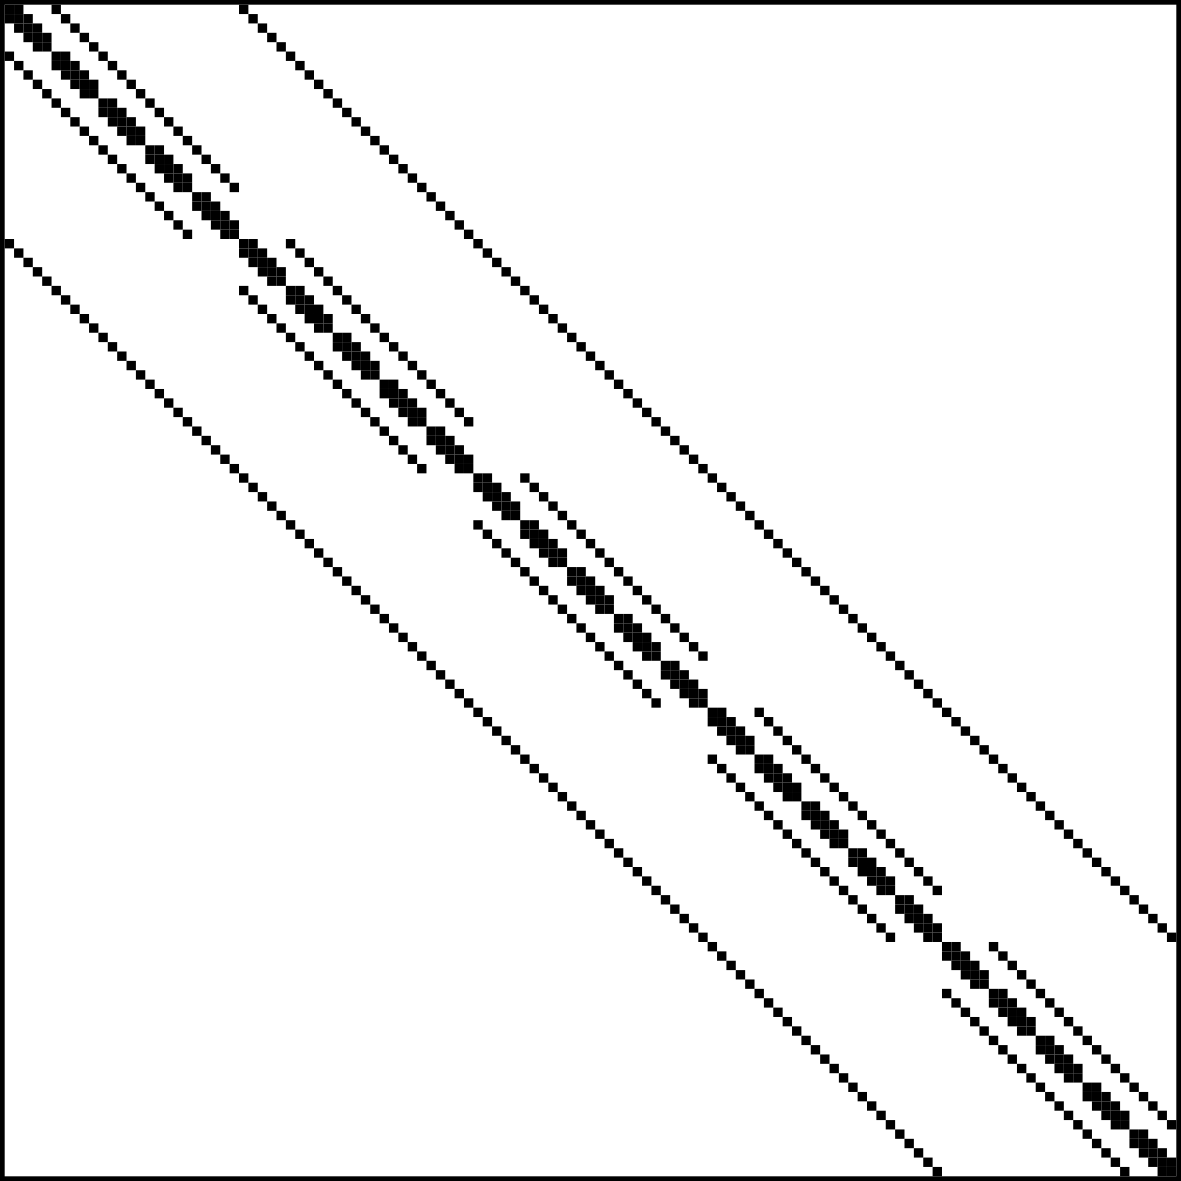
\includegraphics[width=1.0\textwidth]{fig/laplacian_example.png} % second figure itself
        \end{minipage}
        \toccaption{Structured grid and corresponding sparse banded matrix for a simple Laplacian.}{This exemplary
          sparse banded matrix derived from a grid with edge size $d=5$ is representative of the matrices used in this
          chapter to characterize the C3SR-format's storage scheme and benchmark its arithmetic performance.}
        \label{fig:laplacian-example-reprint}
    \end{figure}

    Given a fixed grid edge size $d$, the two corresponding matrices from both families differ only in their nonzeros'
    numerical values. The first matrix family's nonzeros are all identical while for the second family no two nonzeros
    share the same numerical value. This means that in addition to the ability to highly compress the matrix's
    structure, the C3SR-format also allows to store the nonzeros' values of matrices from the first family very
    compactly. This latter option is prohibited by the second matrix family's choice of values.

    The choice of matrices has been made to mimic the properties of real problems, where a structured grid's sparse
    banded matrix's nonzero values, i.e. the weights of connections between neighboring nodes, are determined by
    evaluating a continuous scalar field $\phi: \mathbb{R}^3 \rightarrow \mathbb{R}$ at the midpoint between the two
    nodes in question. An exemplary scalar field, which has been used in this project beforehand, is
    $$
    \phi_{\vec{n}}(\vec{r}) = 2+
      \sin\bigg(\frac{r_x}{d_x}\cdot \pi \cdot n_x \bigg)+
      \sin\bigg(\frac{r_y}{d_y}\cdot \pi \cdot n_y \bigg)+
      \sin\bigg(\frac{r_z}{d_z}\cdot \pi \cdot n_z \bigg)
    $$

    where $d_i$ denotes the grid's edge size in each dimension, and incidentally also the grid's span if its origin is
    placed at the coordinate system's origin. $\vec{n}$ is a parameter determined by the underlying physical problem.
    Thus, in general for most problems no two rows' nonzeros will exhibits the same values and the C3SR-matrix's values
    array V will be densely populated. This configuration corresponds to the second family of matrices. Nevertheless
    there exist problems which yield $\vec{n} \equiv 0$ which causes all nonzeros to be equal meaning that the
    C3SR-format will store them very economically. This case corresponds to the first family of matrices.

    To avoid thinking about the matrix in terms of countless unwieldy calculations, the scalar field approach has been
    dropped in favor of the simplified notions introduced above. The salient characteristics of the matrices that matter
    for this project are that both types share the same structure and that the nonzeros of one type of matrix can be
    compressed while those of the second type cannot. This is equally well achieved by the methods used here which, as
    an additional benefit, entail a speedup during construction of the original CSR-matrix object as the computations
    for evaluating the scalar field are elided.

    Figure \ref{fig:test-matrices-object-size} shows the total matrix object size for a range of grid edge sizes and for
    both families. Note that for a given grid edge size $d$ the matrix objects' sizes vary hugely between the two
    families. This is solely due to the difference in the sizes of the values array V. The exact composition of the
    objects' total size will be examined in detail in the next section.

    \begin{figure}[H]
        \centering
        \captionsetup{width=0.9\columnwidth}
        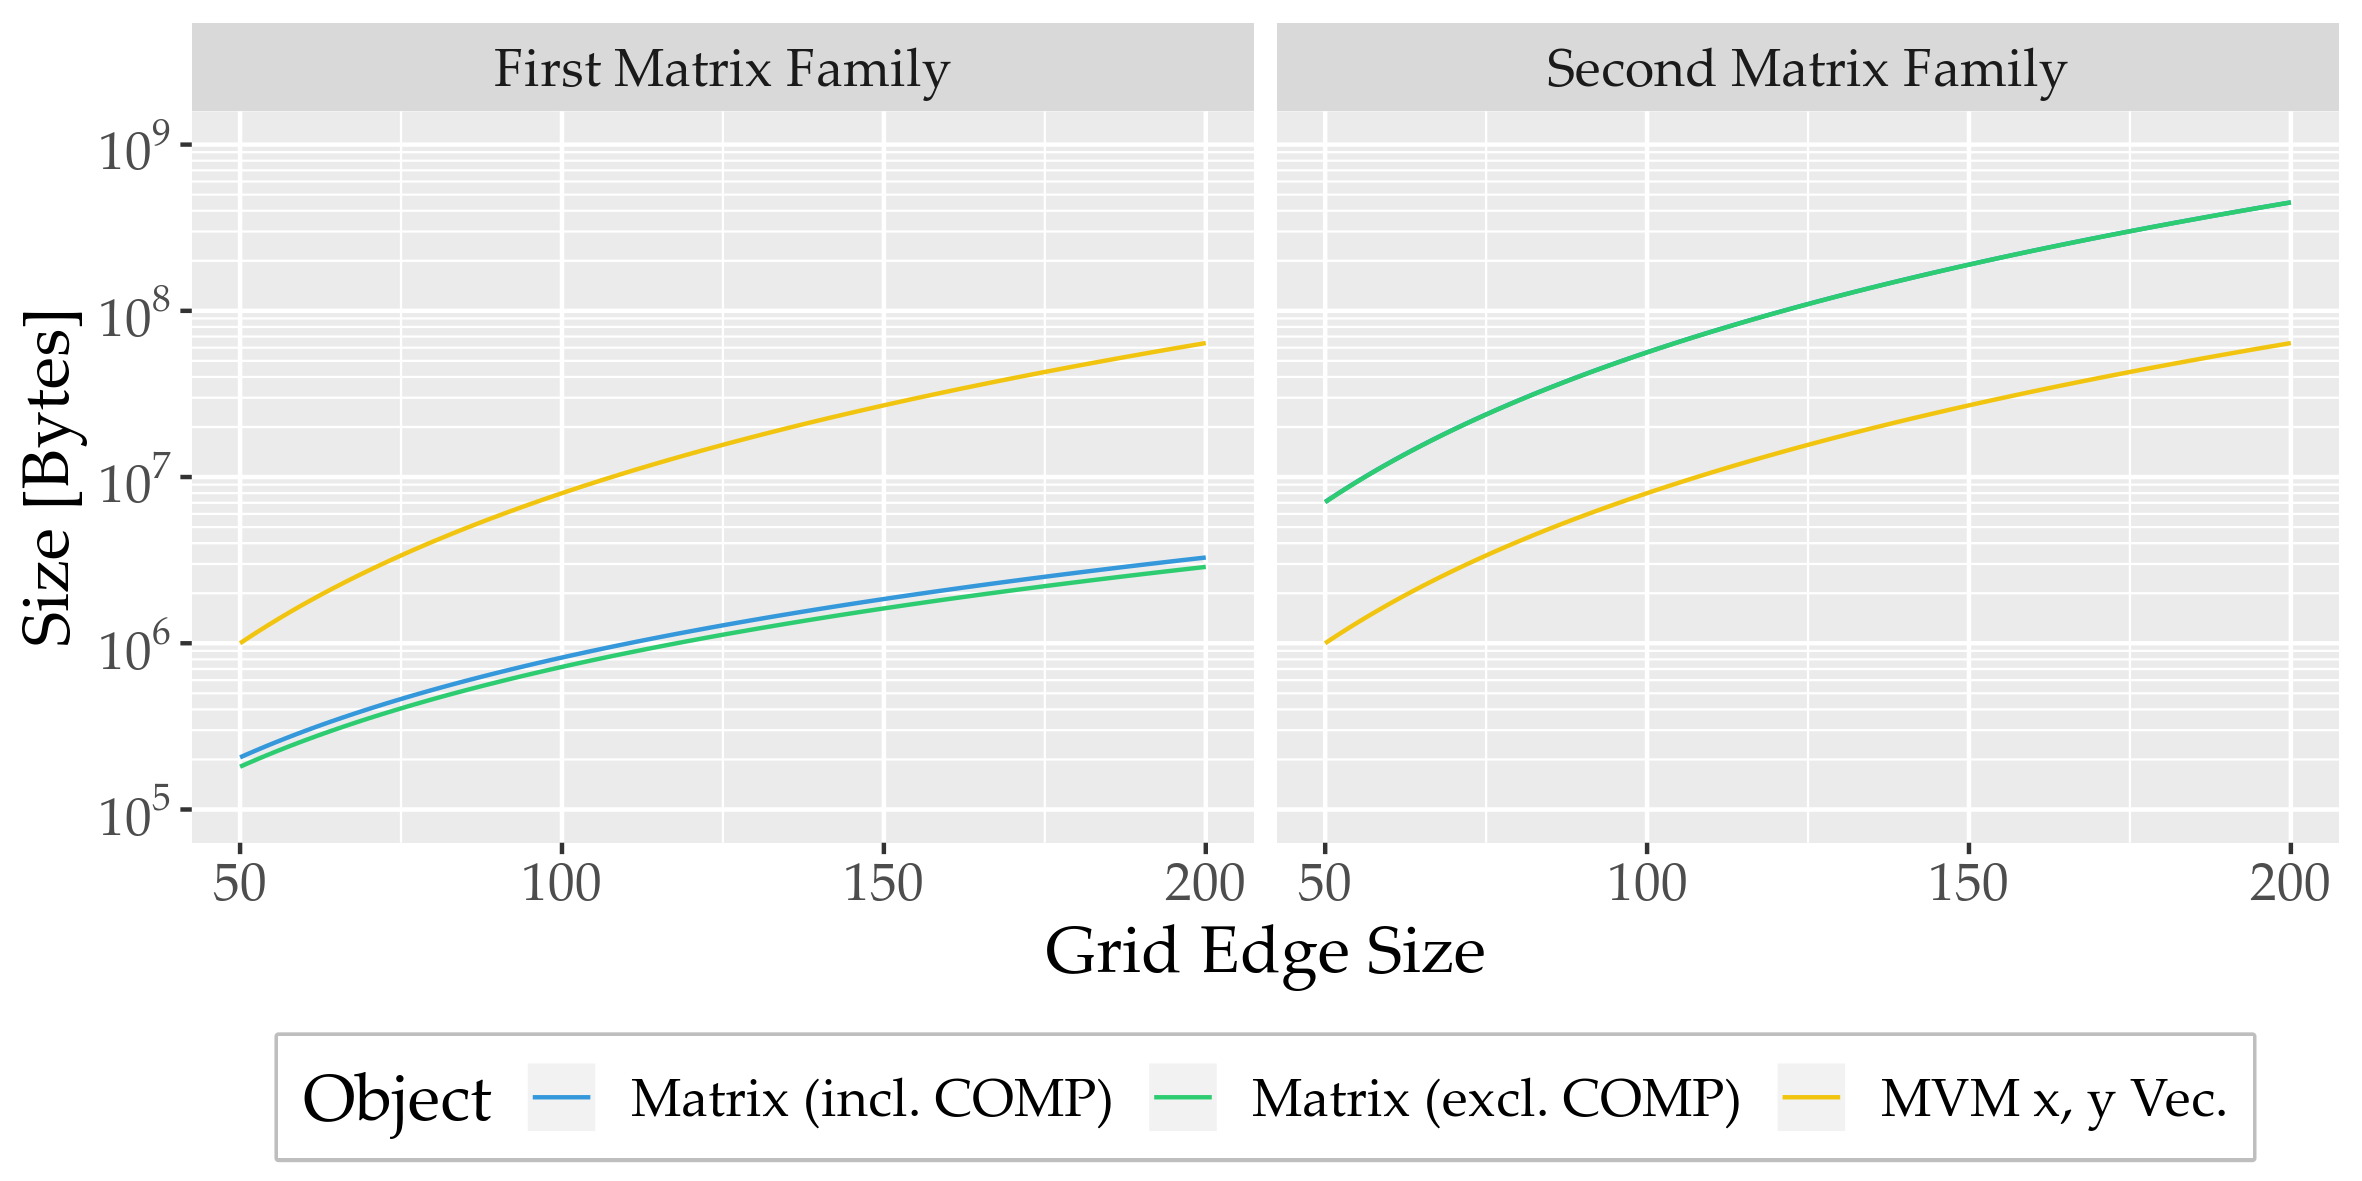
\includegraphics[width=0.9\columnwidth]{assets/test-matrices-object-size.png} % second figure itself
        \toccaption{Measured C3SR-matrix object sizes for both types of families depending on the underlying grid's edge
          size $d$.}{Matrix object sizes including and excluding the COMP array are shown for comparison. Their
          difference is very small and cannot be resolved for the second family's plot. Thus, for all intents and
          purposes the COMP object's size contribution can be ignored. Additionally, for later reference, the storage
          sizes of the dense argument vector $x$ and the dense output vector $y$ of a matrix-vector multiplication $A
          \cdot x = y$ are plotted alongside the matrix object's size. As the matrix is square $dim(x) = dim(y)$ and
          thus both vectors require the same storage space.}
        \label{fig:test-matrices-object-size}
    \end{figure}

    The C3SR-matrix objects are created from the matrix's corresponding object in CSR-format according to the methods
    explained in Section \ref{sec:gen-of-c3sr-from-csr}. The CSR-matrices are created using Matrixgen, a sparse matrix
    creation toolkit, which has been developed alongside the C3SR-format project as an aid to its development. Matrixgen
    is briefly showcased in Part II of this thesis.

  \section{Relative Object Size for Fully Structured Matrices} \label{sec:rel-object-size-fully-structured}

    An insightful characteristic of a sparse matrix format is its object's storage space divided by the number of
    nonzeros in the matrix referred to as the \keyword{relative object size}. As previously stated, matrix-vector
    multiplication usually is a memory-bound operation and thus reducing the matrix's object size improves performance
    by limiting the amount of data that is required to move for the computation. As opposed to evaluating absolute
    object sizes, which are rather abstract without explicit knowledge of their context, the relative object size
    constitutes an intuitive heustic and can be conceived of as a `price' one has to pay for any additional nonzero.

    Using matrices from the two families introduced in the previous section their relative object sizes are examined as
    a function of the grid's edge size and are compared against the corresponding matrix object in CSR-format. The COMP
    array is be considered to be a part of the object regardless of the circumstance, that it's an asset solely used for
    vectorized matrix-vector multiplication. Analytical convergence values are derived for all configurations and
    corresponding measurement results are shown thereafter.

    \paragraph{Relative Storage Size for Matrices in CSR-Format}

    The CSR format's storage requirements are identical for both matrix families as they differ only in their nonzero's
    numerical values. Per nonzero one element is stored in the values array and in the column-index array in addition to
    one entry to the row-pointer array per matrix row. As for large matrices the vast majority of rows corresponds to
    inner nodes which all have $7$ nonzeros, or more formally, $\lim \limits_{d\rightarrow \infty}
    \frac{n_{\text{nnz}}}{n_{\text{row}}} = 7$. The number of rows can thus be expressed in terms of the number of
    nonzeros in the limit $d \rightarrow \infty$ and hence the storage requirements per nonzero amount to the following
    value:

    \begin{center}
      \begin{tikzpicture}
        \node[draw=dodgerblue4, inner sep=0.4cm, font=\Large] (EQ)
        {
          $
          \lim \limits_{d \rightarrow \infty}\frac{n_{\text{Bytes}}}{n_{\text{nnz}}}
          = \frac{\overbrace{(8 + 4) \cdot n_{\text{nnz}}}^{\text{V + CI}} + \overbrace{4 \cdot n_{\text{row}}}^{\text{RP}}}{n_{\text{nnz}}}
          = 12 + 4\cdot \lim \limits_{d \rightarrow \infty} \frac{n_{\text{nnz}}}{n_{\text{nrow}}}
          = 12 + \frac{4}{7}
          \approx 12.57
          $
        };
        \node[draw=dodgerblue4, fill=dodgerblue4, text=white, anchor=south west, inner sep=0.2cm] (WHAT)
          at (EQ.north west)
          {$1^{\text{st}}$ and $2^{\text{nd}}$ Matrix Family in CSR-Format};
      \end{tikzpicture}
    \end{center}

    \paragraph{Relative Storage Size for Matrices in C3SR-Format}

    In order to analyze the relative storage requirements of the corresponding objects in C3SR-format the sizes of the
    individual data arrays must be examined. By design, matrices with unique values produce one element per nonzero in
    the values array V. J encodes the unique adjacency patterns of the matrix's nodes and thus locks in at $135$ elements for
    any $d \geq 3$, produced by the $8$ corners a $4$ neighbors, $12$ edges a $5$ neighbors, $6$ faces a $6$ neighbors
    and the inner nodes with $7$ neighbors each. In smaller grids one or more unique node classes are not present.

    Every node in a contiguously indexed set of inner nodes produces a contiguous segment of $7$ unique values within V
    and hence the index-pointers $vs_i$ in VS increase at a fixed increment of $7$ for these nodes, which allows the
    segment within VS to be condensed into a single run-length-increment encoded triplet, as illustrated in Figure
    \ref{fig:rlei-encoding-of-vs}. The constant stride offset between the $d-2$ elements $vs_i$ is eventually
    interrupted at the grid's border where the corresponding matrix rows have fewer nonzeros. Thus, with exceptions
    arising at rows corresponding to nodes at the $y$- and $z$-borders, VS chiefly consists of blocks of two
    RLI-triplets: the first for a contiguous segment of $d-2$ inner nodes as explained above followed by another triplet
    encoding the two nodes at the $x=d-1$ and $x=0$ boundaries, prefacing the next contiguous segment of inner rows. In
    total, there are $(d-2)^2$ such block pairs. Consider Figure \ref{fig:laplacian-example-reprint} as an example: The
    first contiguous segment of inner rows comprises indices $\{32, 33, 34\}$ and is followed by the boundary nodes
    $\{35, 36\}$. The next contiguous segment then follows at index $37$ etc.

    \begin{figure}[H]
      \centering
      \captionsetup{width=0.9\textwidth}
      \begin{tikzpicture}[
        node distance=1cm and 0.1cm,
        vsstyle/.style={draw=gray, minimum height=1cm, minimum width=3cm, fill=dodgerblue4, text=white},
        vstyle/.style={draw=gray, minimum height=1cm, minimum width=3cm},
        pathstyle/.style={->}
      ]
        \node[circle, draw=gray] (VNAME)
          {V};
        \node[anchor=west, right=of VNAME] (DOTS1)
          {$\cdots$};
        \node[vstyle, right=of DOTS1, anchor=west] (VK)
          {$v_{k}$};
        \node[right=of VK, anchor=west] (DOTS2)
          {$\cdots$};
        \node[vstyle, right=of DOTS2, anchor=west] (VKP7)
          {$v_{k+7}$};
        \node[right=of VKP7, anchor=west] (DOTS4)
          {$\cdots$};
        \node[right=of DOTS4, anchor=west] (DOTS5)
          {$\cdots$};
        \node[vstyle, right=of DOTS5, anchor=west] (VKD)
          {$v_{k+7\cdot((d-1) - 2)}$};
        \node[right=of VKD, anchor=west] (DOTS6)
          {$\cdots$};

        \node[circle, anchor=center, fill=dodgerblue4, text=white, draw=gray] (VSNAME)
          at ($(VNAME)+(0,-2.0)$)
          {VS};
        \node[anchor=west] (VSDOTS1)
          at ($(VSNAME.east)+(0.5,0)$)
          {$\cdots$};
        \node[vsstyle, right=of VSDOTS1] (VSR)
          {$vs_r$};
        \node[vsstyle, right=of VSR] (VSRP1)
          {$vs_{r+1}$};
        \node[right=of VSRP1] (VSDOTSVSRP1)
          {$\cdots$};
        \node[vsstyle, right=of VSDOTSVSRP1] (VSRPDM2)
          {$vs_{r + ((d-1)-2)}$};
        \node[right=of VSRPDM2] (VSDOTSVSRPDM2)
          {$\cdots$};

        \node[anchor=north, text=dodgerblue4, inner sep=0.2cm, fill=gray!15, draw=dodgerblue4] (TRIPLET)
          at ($(VSDOTSVSRP1.south)+(0, -2)$)
          {$\big(r, k, 7\big)$};

        \draw[pathstyle] (VSR.north) |- ($(VSR.north)!0.5!(VK.south)$) -| (VK.south);
        \draw[pathstyle] (VSRP1.north) |- ($(VSRP1.north)!0.5!(VKP7.south)$) -| (VKP7.south);
        \draw[pathstyle] (VSRPDM2.north) |- ($(VSRPDM2.north)!0.5!(VKD.south)$) -| (VKD.south);
        \draw[] (TRIPLET.north) -- (VSR.south);
        \draw[] (TRIPLET.north) -- (VSRP1.south);
        \draw[] (TRIPLET.north) -- (VSRPDM2.south);
        \draw[] (TRIPLET.north) -- (VSRPDM2.south);
        \draw[shorten >= 0.2cm] (TRIPLET.north) -- (VSDOTSVSRP1.south west);
        \draw[shorten >= 0.2cm] (TRIPLET.north) -- ($(VSDOTSVSRP1.south west)!0.5!(VSDOTSVSRP1.south)$);
        \draw[shorten >= 0.2cm] (TRIPLET.north) -- (VSDOTSVSRP1.south);
        \draw[shorten >= 0.2cm] (TRIPLET.north) -- ($(VSDOTSVSRP1.south east)!0.5!(VSDOTSVSRP1.south)$);
        \draw[shorten >= 0.2cm] (TRIPLET.north) -- (VSDOTSVSRP1.south east);
      \end{tikzpicture}
      \toccaption{Section within V and VS pertaining to a contiguous segment of inner nodes for matrices from the second
        family.}{Pointer-index values $vs_i$ are indicated by arrows to the elements they point. Inner nodes yield matrix
        rows with 7 nonzeros and thus the corresponding section of VS comprises $d-2$ contiguous elements whose values
        increase at a constant stride of $7$. This constellation is efficiently condensed into a single
        run-length-increment encoded triplet.}
      \label{fig:rlei-encoding-of-vs}
    \end{figure}

    Similarly to the constellation created by contiguous inner nodes any set of contiguous nodes at the grid's faces or
    edges can be compressed into two or three RLI-triplets. However, as their number grows linearly with $d$ compared to
    $d^2$ for the grid's inner volume their effects become minute for larger $d$ and are of no consequence to
    convergence behavior.

    JS exhibits the very same structure as VS, consisting mainly of pairs of RLI-triplets which correspond to contiguous
    inner nodes. All inner nodes exhibit the same pattern, hence all corresponding $js_i$ point the same element in $J$,
    producing a single RLI-triplet followed by a second one for the two following border nodes. In contrast to $VS$,
    whose $vs_i$ exhibit a stride of $7$ between inner nodes, the $js_i$ exhibit no offset equal to a stride of $0$
    which thus allows them to be run-length-increment encoded in just the same manner. RS is subject to the very same
    reasoning as JS: Nodes in the inside of the grid produce slices of rows with $7$ nonzeros each, interrupted by nodes
    at the grid boundaries. 

    As exemplified in Figure \ref{fig:laplacian-example-reprint} nodes at any $z > 0$ are adjacent to another node
    situated below them in negative $z$-direction and thus the peg indices of two adjacent nodes at $z > 0$ are offset
    by $1$ carrying on for all following nodes. Hence the peg indices for all nodes with $z > 0$ are condensed into a
    single RLI-triplet. Similarly for $z = 0$ all nodes at $y > 0$ are stored by single RLI-triplet leaving, at worst,
    $d$ further triplets to be stored for the remainder of the matrix.
 
    Finally, the COMP array requires $\mathcal{O}(d^2)$ bytes due to reasoning analogous to that pertaining to VS, JS
    and RS: SIMD chunks across inner nodes all produce the same composition yielding a single RLI-triplet followed by
    disturbances of this regularity at the grid's boundaries, after which the next chunk of rows corresponding to inner
    nodes is arrived at.

    Collating the above results yields that none of the data arrays except V require storage size larger than
    $\mathcal{O}(d^2)$. As $n_{\text{nnz}} \rightarrow 7\cdot d^3$ for increasing $d$ the storage size per nonzero
    converges to 8 for the second family of matrices, which is characterized by fully unique nonzeros.

    \begin{center}
      \begin{tikzpicture}
        \node[draw=dodgerblue4, inner sep=0.4cm, font=\Large] (EQ)
        {
          $
          \lim \limits_{d \rightarrow \infty}\frac{n_{\text{Bytes}}}{n_{\text{nnz}}}
          = \frac{\overbrace{8 \cdot n_{\text{nnz}}}^{\text{V}} +
                  \overbrace{\mathcal{O}(1)}^{\text{J}} +
                  \overbrace{\mathcal{O}(d^2)}^{\text{VS}} +
                  \overbrace{\mathcal{O}(d^2)}^{\text{JS}} +
                  \overbrace{\mathcal{O}(d^2)}^{\text{RS}} +
                  \overbrace{\mathcal{O}(d)}^{\text{JP}} +
                  \overbrace{\mathcal{O}(d^2)}^{\text{COMP}}}{n_{\text{nnz}}}
          = 8
          $
        };
        \node[draw=dodgerblue4, fill=dodgerblue4, text=white, anchor=south west, inner sep=0.2cm] (WHAT)
          at (EQ.north west)
          {$2^{\text{nd}}$ Matrix Family in C3SR-Format};
      \end{tikzpicture}
    \end{center}

    Considering matrices from the first family, whose nonzeros are all identical, note that the total number of elements
    in V is limited by unique classes of nodes in the grid, just as described above for J. In the same manner the
    storage requirements for $V$ are constant for all $d > 3$ and thus in $\mathcal{O}(1)$. Due to this VS exhibits the
    same configuration as JS in the case layed out above. J, JP and RS remain unchanged while COMP retains its storage
    size requirements of $\mathcal{O}(d^2)$. The composition of SIMD chunks across inner nodes only changes its type
    according to the new data layout. Thus the relative storage requirements of matrices from the first family, whose
    nonzeros are all identical, converges towards $0$.

    \begin{center}
      \begin{tikzpicture}
        \node[draw=dodgerblue4, inner sep=0.4cm, font=\Large] (EQ)
        {
          $
          \lim \limits_{d \rightarrow \infty}\frac{n_{\text{Bytes}}}{n_{\text{nnz}}}
          = \frac{\overbrace{\mathcal{O}(1)}^{\text{V}} +
                  \overbrace{\mathcal{O}(1)}^{\text{J}} +
                  \overbrace{\mathcal{O}(d^2)}^{\text{VS}} +
                  \overbrace{\mathcal{O}(d^2)}^{\text{JS}} +
                  \overbrace{\mathcal{O}(d^2)}^{\text{RS}} +
                  \overbrace{\mathcal{O}(d)}^{\text{JP}} +
                  \overbrace{\mathcal{O}(d^2)}^{\text{COMP}}}{n_{\text{nnz}}}
          = 0
          $
        };
        \node[draw=dodgerblue4, fill=dodgerblue4, text=white, anchor=south west, inner sep=0.2cm] (WHAT)
          at (EQ.north west)
          {$1^{\text{st}}$ Matrix Family in C3SR-Format};
      \end{tikzpicture}
    \end{center}

    \paragraph{Measurement Results}

    A measurement of the relative object size is displayed in \ref{fig:bytespernnz} for a wide range of values of $d$
    and both families of matrices, comparing the CSR- and C3SR-format. The measured values are shown to converge very
    rapidly toward their respective analytical limits determined above. Matrices from the first family reach relative
    storage sizes of less than $1/10$ bytes per nonzero even for fairly small grid dimensions with values much lower for
    larger grids. Second family matrices, whose nonzeros all differ, reach convergence towards $8$ bytes per nonzero
    at tiny grid sizes of $\leq 50$. This means, that for the latter case the vast majority of storage space is spent
    for the nonzeros' values while the matrix structure is represented almost free of charge. In the other case, where
    the nonzeros are compressed, the compression scheme is powerful enough to approach the limit of vanishing storage
    costs.

    \begin{figure}[H]
      \centering
      \captionsetup{width=0.9\textwidth}
      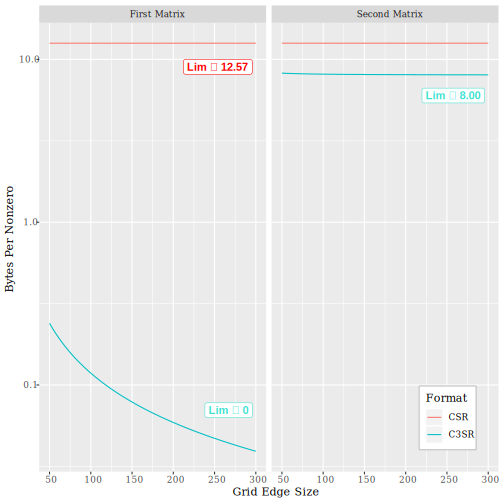
\includegraphics[width=0.9\textwidth]{assets/bytespernnz}
      \toccaption{Measured object storage size per nonzero matrix element for the two families of sparse banded matrices
        derived from fully structured grids for the CSR- and C3SR-formats.}{Analytical convergence limits for $d
        \rightarrow \infty$ are annotated next to each curve. The CSR's values are identical for both matrix families
        and the corresponding curve has been annotated only once. The matrix families correspond to the problem
        exemplified by Figure \ref{fig:laplacian-example} and differ only in the values of their nonzero elements, with
        the first family using a single constant value and the second family using unique values for each nonzero.
        Nonzeros are stored as 8-byte double precision floats while indices are stored as 4-byte integers. Only values
        for $d \geq 50$ are displayed for the sake of legibility, as the overhead of the C3SR format's compression
        scheme yields very large relative storage size requirements for small matrices. The C3SR-matrix object's size
        includes the COMP array.}
      \label{fig:bytespernnz}
    \end{figure}

    It should be noted that the matrices tested in this section present ideal use cases around which the C3SR-format was
    conceived. The effects of deviations from this ideal will be explored in the next section by introducing
    perturbations to the regularity of the matrices. Nevertheless the results show the C3SR-format to be a zero-cost
    compression scheme in that whichever aspect of a sparse banded matrix derived from a structured grid can be
    compressed, numerical values or structure, compresseses perfectly in the above sense.

  \section{Object Size per Nonzero for Perturbed Structured Matrices} \label{sec:objsize-perturbed}

    In contrast to the fully structured matrices examined in the previous section many real-life problems produce
    matrices whose structure exhibits deviations from the ideal in individual, non-contiguous rows. Such configurations
    may arise where the underlying mathematical problem entails integration over $1$- or $2$-dimensional manifolds in
    $3$-dimensional domains. These manifolds intersect the grid along nodes whose indexing is not contiguous introducing
    perturbations to the regularity of the resulting linear system's coefficient matrix at seemingly random positions of
    rows. See Figure \ref{fig:structured-grid-with-path} for an illustration of this notion.

    \begin{figure}[H]
      \centering
      \captionsetup{width=0.9\textwidth}

      \toccaption{Structured grid with integration path over non-contiguous nodes and corresponding matrix.}
        {?? 2D 10x10 Grid mit Integrationspfad und korresp. Matrix mit Störungen. \todo{s}}
      \label{fig:structured-grid-with-path}
    \end{figure}

    In order to gauge the stability of the C3SR-format's compression scheme to such configurations, which can be
    considered as slight deviations from the best-case scenario, the experiment performed in the previous section is
    repeated with perturbations introduced into the matrices. Choosing random matrix rows, their nonzeros' values and
    positions within the row are randomized. The values are drawn from a uniform distribution over the half-open
    interval $[1, 2)$ while the column indices are randomly selected from all possible column index values without
    duplication. Given a grid with edge size $d$ and its initial, unperturbed matrix the relative storage density as
    bytes per nonzero is measured while varying the relative ratio of matrix rows to perturb. The experiment is repeated
    to account for its stochastic aspect.

    Measurement results for two samples of matrices, based on a small and a larger grid, $d = 50$ and $d = 200$, and
    perturbations of up to $10\%$ of matrix rows are showcased in Figure \ref{fig:bytespernnz-perturbed}. Both families
    of matrices are shown to be very stable with respect to increasing ratios of perturbed rows. Matrices from the
    second family display a decrease in storage density of approximately $1\%$ per $1\%$ increase in the relative number
    of perturbed rows. A separate measurement reveals that the C3SR-format surpasses the CSR-format in storage density
    even if $75\%$ of matrix rows are randomized in the manner explained above and only the remaining $25\%$ are
    retained in their original, structured form. While matrices from the first family show a much greater decrease in
    storage density, their absolute values are very small, reaching approximately $2$ bytes per nonzero at $10\%$
    perturbed rows. Except for different starting points of the unperturbed matrices, their underlying grid's size does
    not have any qualitative impact.

    \begin{figure}[H]
      \centering
      \captionsetup{width=0.9\textwidth}
      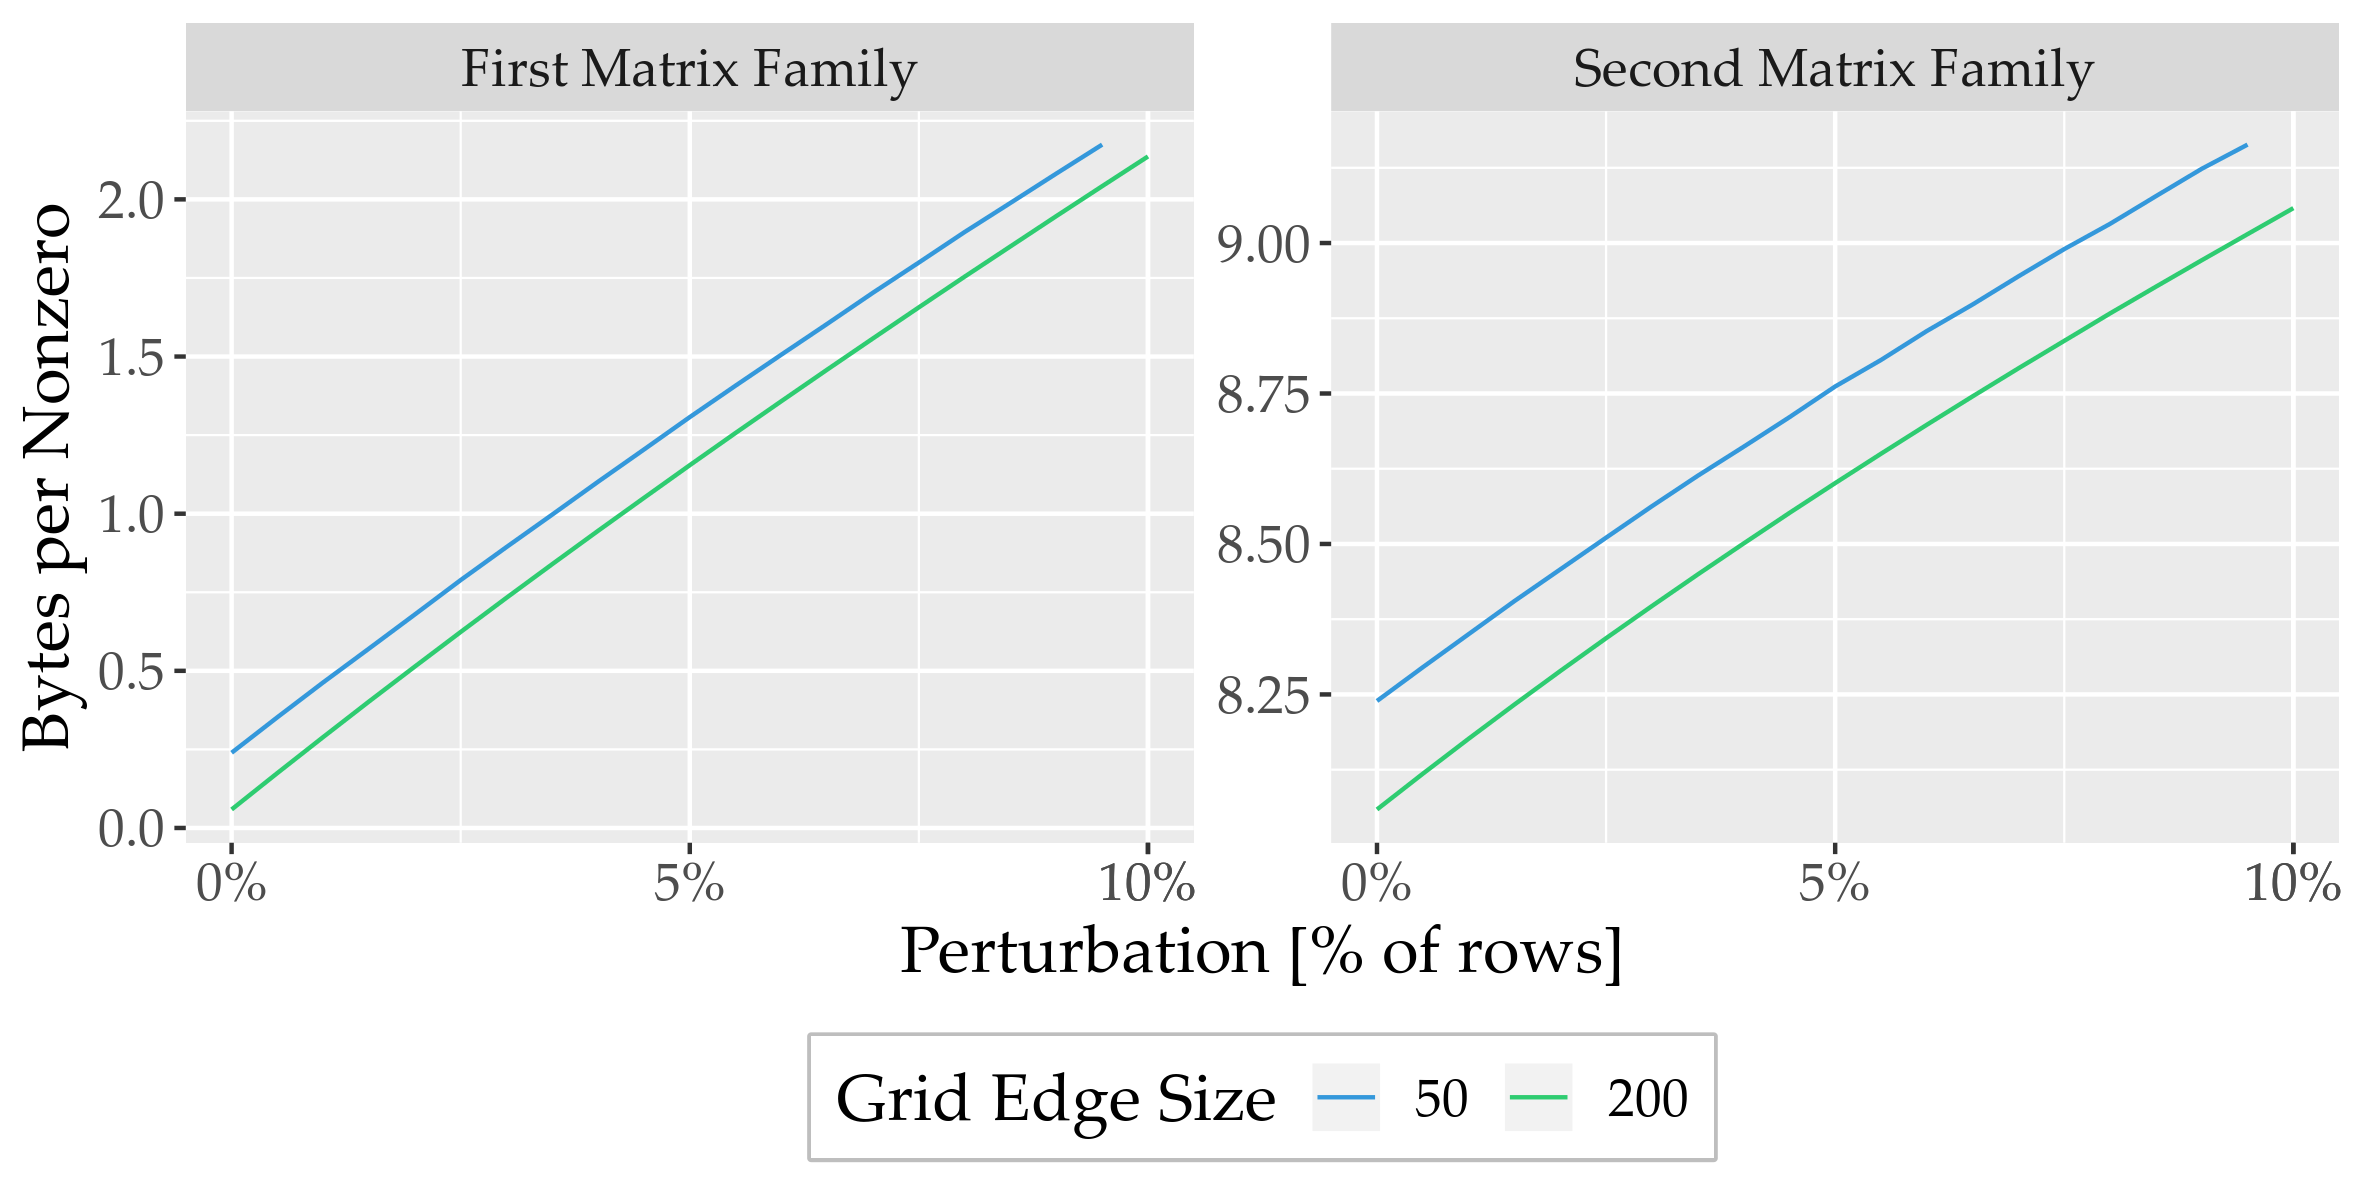
\includegraphics[width=0.9\textwidth]{assets/bytespernnz-perturbed}
      \toccaption{Measurement of the relative storage sizes of two sets of perturbed sparse banded matrices from the two
        matrix families.} {For each family two matrices corresponding to two different grids are perturbed by
        randomizing a portion of their rows. Each perturbed row has its nonzeros' positions shuffled and their numeric
        values randomized. The matrix objects relative storage size is measured as a gauge of the C3SR-format's
        stability to perturbations from the ideal configuration. The graphs display mean values over 1000 iterations for
        each degree of perturbation. All respective standard deviations are smaller than $1\%$ of their correpsonding
        mean values and have been omitted from the graph.}
      \label{fig:bytespernnz-perturbed}
    \end{figure}

    The decrease in storage density is owed to the fact that a perturbed row's column indices are randomized,
    effectively increasing the pattern array J by $7$ elements and, for the first family of matrices whose values array
    V is essentially empty, also adding $7$ new unique values to V. Due to the fact, that the second family of matrices'
    V array is by far the largest of all of its data arrays, and because V does not increase in size as the values are
    uncompressible in the first place, randomizing a row has less effect than for first family matrices, explaining the
    difference in the decrease in storage density. In addition, run-length-increment encoding of the structural
    information of contiguous rows corresponding to segments of contiguous inner nodes is inhibited by every randomized
    matrix row within the segment for both matrix families.

    \Todo{Fazit: Stable against small perturbations}

  \section{Matrix-Vector Multiplication of Fully Structured Matrices} \label{sec:mvm-structured}

    Analogous to the examination of the C3SR-format's storage density its arithmetic performance of matrix-vector
    multiplications is assessed for fully structured matrices and for matrices derived from slightly perturbed
    structured grids. Three machines were used to benchmark execution times: 

    \begin{itemize}[leftmargin=5cm]
      \item[\textbf{mp-knl4}] {Knights Landing Architecture, 1 socket à 64 cores, 4 NUMA regions}
      \item[\textbf{mp-skl2s24c}] {Skylake SP Architecture, 2 sockets à 24 cores, 4 NUMA regions}
      \item[\textbf{mp-skl2s8c}] {Skylake SP Architecture, 2 sockets à 8 cores, 2 NUMA regions} 
    \end{itemize}

    Detailed specifications for each machine and its architecture is available at the \href{\ascWiki}{ASC Server
    Hardware Wiki}. The systems' salient characteristics relevant to the results presented in this section are mentioned
    as they are needed. 

    Execution times were measured for both multiplication flavors introduced in Section
    \ref{subsec:matrix-vector-multiplication-schemes}, the scalar, CSR-like scheme and the vectorized scheme based on
    SIMD operations. The two flavors will be abbreviated as \keyword{csrpar} and \keyword{simdpar} named according to
    their implementation and the fact that they are fully parallelized across the system's cores. Parallelization is
    parameterized by row index, i.e. the index-space $\{0, \ldots, n_{\text{rows}} - 1\}$ is spread evenly amongst the
    threads $\{0, \ldots, n_\text{threads} - 1\}$. For the matrices studied herein this suffices to account for
    NUMA-locality according to the explanation given in the previous chapter. The achieved bandwidth is then determined
    as the quotient of the total amount of moved data and the duration required. The data read from memory is comprised
    of the matrix object and the argument vector while data is written exclusively to the output buffer as previously
    shown in Figure \ref{fig/test-matrices-object-size}.

    As a guage of quality an upper limit to the achievable bandwidth was determined from each machine's read and write
    bandwidth and the total amounts of data read and written. The memory accesses involved in the arithmetic of the
    matrices studied herein are relatively structured and regular such that the assumption is made that each section of
    memory is read only once from main memory and that if data is required at multiple times during execution it can be
    retrieved from cache memory. Using the notation of $d_r$ and $d_w$ for the data read and written, and $b_r$ and
    $b_w$ for the read and write bandwidths, the achievable $b_\text{max}$ limit can be expressed as
    $$
      b_{\text{max}} = \frac{d_r + d_w}{\frac{d_r}{b_r} + \frac{d_w}{b_w}}
    $$

    The above expression is immediately derived from $t_\text{max} = t_r + t_w$ where $t_i$ are the corresponding
    operations' durations which can be stated in terms of bandwidths via $t_i = d_i / b_i$. The systems' read and write
    bandwidths are determined using the benchmark suite Likwid Bench \cite{likwidbench:github} by performing AVX512 load
    and store instructions at full system capacity for a fixed volume of data. The obtained values are as follows:

    \begin{center}
    \begin{tabular}{r|c|c}
      \textbf{Machine} & \textbf{Read Bandwidth} & \textbf{Write Bandwidth} \\
      \hline
      mp-knl4     & 292 GB/s & 156 GB/s \\
      mp-skl2s24c & 230 GB/s & 72 GB/s  \\
      mp-skl2s8c  & 120 GB/s & 60 GB/s  \\
    \end{tabular}
    \end{center}

    Note that these bandwidths refer to the type of memory required to hold all of the objects involved in a
    matrix-vector multiplication for the largest problem types based on grids with edge sizes of $d = 200$ nodes. For
    the Skylake machines this corresponds to main memory while the KNL's high-bandwidth memory is still large enough to
    contain all data. 

    Figure \ref{fig:mvm-perturbed-new} displays the obtained benchmark results for both families of matrices derived
    from structured grids.

    \begin{figure}[H]
      \centering
      \captionsetup{width=0.9\textwidth}
      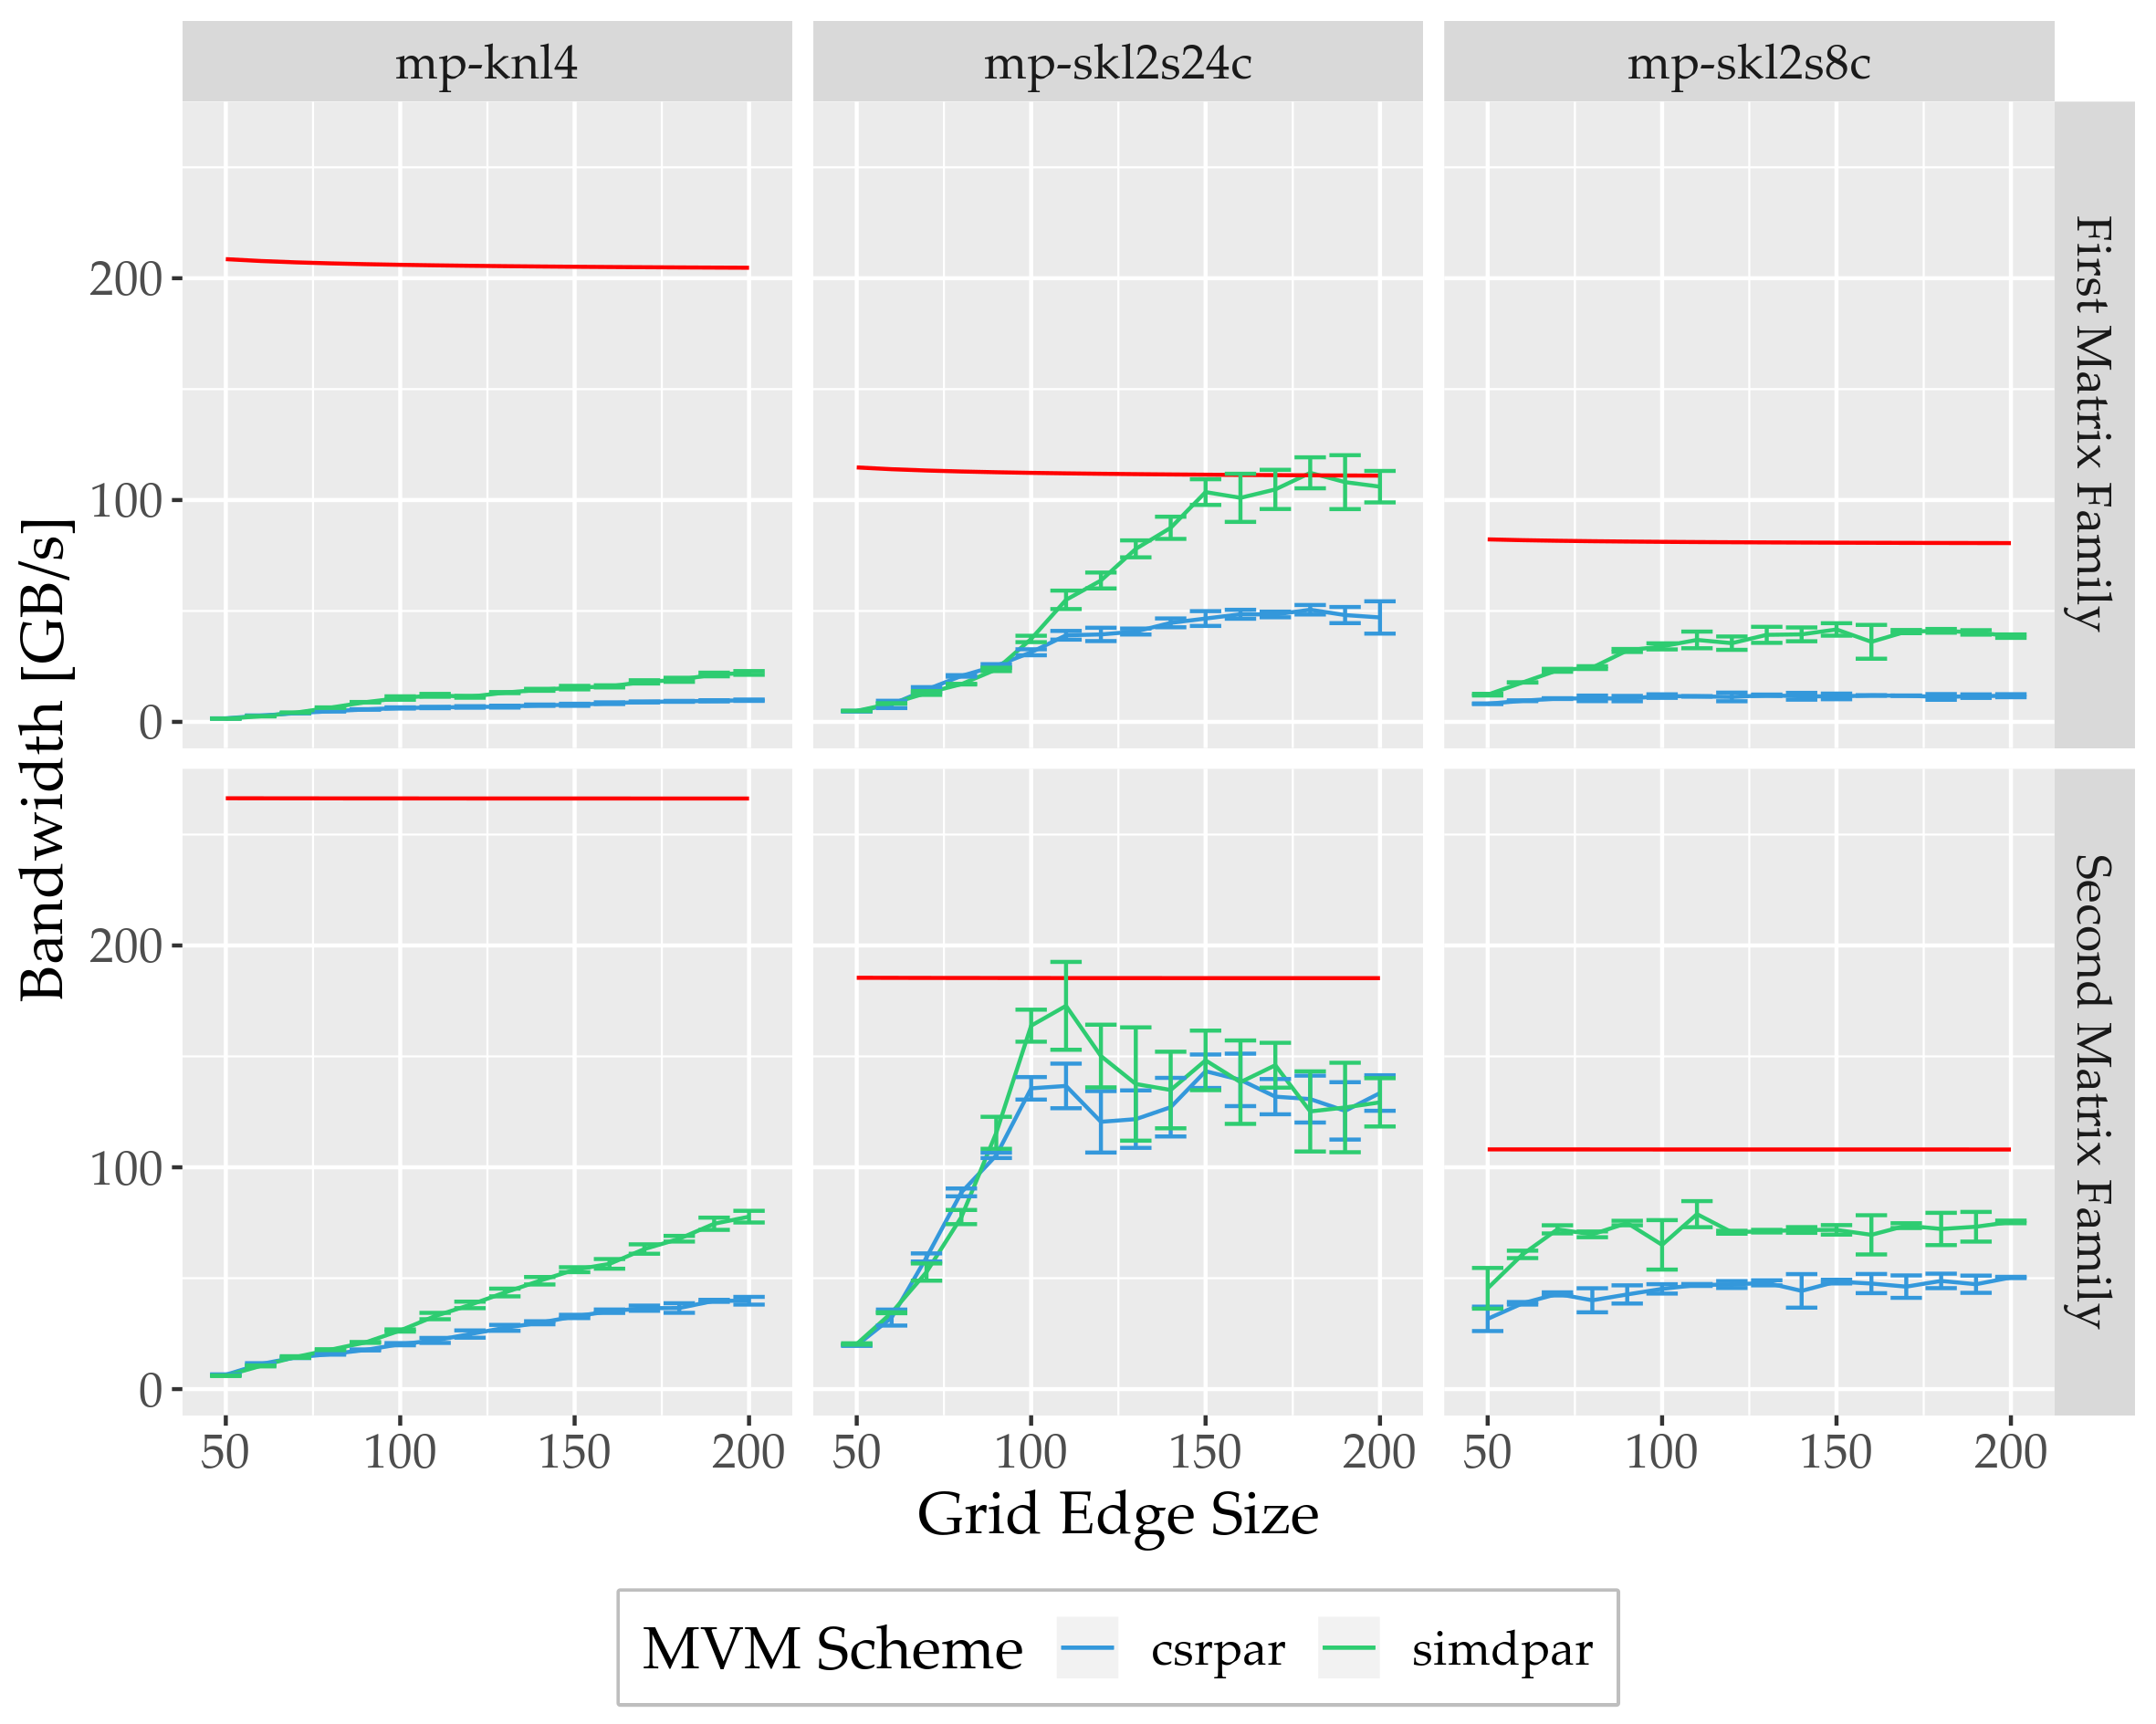
\includegraphics[width=0.9\textwidth]{assets/mvm-perturbed-new}
      \toccaption{todo}{todo}
      \label{fig:mvm-perturbed-new}
    \end{figure}

     In general, the vectorized multiplication scheme is found to be superior except for matrices from the second family
     where the performances of both multiplication schemes are equivalent on the larger Skylake machine. On the same
     machine the bandwidth limit was reached for first family matrices while all other performances maxed out
     significantly below the system bandwidth limits.
 
     The performance of smaller grid sizes is particularly bad and increases as the grid's dimensions are expanded until
     at a certain extent a bandwidth plateau is reached. A separate analysis found the cost of thread synchronization to
     outweight the matrix-vector arithmetic for small problem domains explaining a lack of performance where the
     problem size is not large enough to render the synchronization overhead insignificant. This is reflected in the fact
     the grid size required to reach the bandwidth plateau are larger for first family matrices, as their corresponding
     matrix object's are much lighter resulting in less data movement and faster computation times which, conversely,
     entail a higher relative burden of synchronization.
 
     Additionally, thread synchronization was found to scale poorly with the total number of threads. By this the Knights
     Landing machine is affected severly due to its 64 cores which require larger problem domains to even reach their
     expected bandwidth plateau than were examined for this thesis as is shown in the graphs by the strikingly low
     obtained bandwidth values.
 
     Note that for larger grids $175 \leq d \leq 200$ the measured bandwidths surpass the maximum bandwidth limit by a
     small margin for first family matrices on the larger Skylake machine. The machine is known to produce slightly
     higher bandwidths for composite operations that involve reading from and writing to memory than the plain read and
     write bandwidths would allow. It is suspected that internal latencies of the memory controller can be hidden, at
     least in part, if different memory accesses are issued simultaneously. That means the marked maximum system
     bandwidth is slightly underestimated. Also, the bandwidth overreach for second family matrices on the same machine
     for grids with $d \approx 115$ is a result of the faster L3 cache, which contains all data for this problem and for
     which the bandwidth limit does not apply.
 
     The maximum bandwidth limits appear constant over the complete range of grid edge sizes and for both types of
     matrices. This is owed to the object sizes of the matrix object, the argument vector $x$ and the output vector $y$
     relative to one another. As displayed in Figure \ref{fig:test-matrices-object-size}, for first family matrices
     almost all memory movement involved in a matrix-vector multiplication is due to $x$ and $y$, thus, using the above
     notation, $d_r \approx d_w$. Conversely, for second family matrices the data read is mainly the matrix object whose
     size is a multiple of $y$ and thus $d_r \gg d_w \,\, \land \,\, d_r/d_w \equiv \text{const}$. Based on these
     relations the expressions for the maximum bandwidths simplify to constants:
 
     $$
       b_{\text{max}}^{\text{1st Fam}} = \frac{2}{\frac{1}{b_r} + \frac{1}{b_w}} \quad \quad \quad
       b_{\text{max}}^{\text{2nd Fam}} = \frac{1}{\frac{1}{b_r} + \frac{(d_w/d_r)}{b_w}}
     $$
 
     During development Intel's Threading Building Blocks (TBB) \cite{tbb:github} were intially used for parallelization.
     TBB is a C++ framework for parallel programming which offers implementations of many data types, algorithms and
     synchronization mechanism useful for concurrency. Most of its features transcend the requirements of this project
     while, conversely, other mechanism such as thread pinning are platform specific and require additional libraries.
     The achieved result were unsatisfactory and TBB was ultimately abandoned. Nevertheless, the obtained distribution of
     bandwidths shows a different characteristic which is printed in Figure \ref{fig:mvm-perturbed-old} for direct
     comparison.
 
     \begin{figure}[H]
       \centering
       \captionsetup{width=0.9\textwidth}
       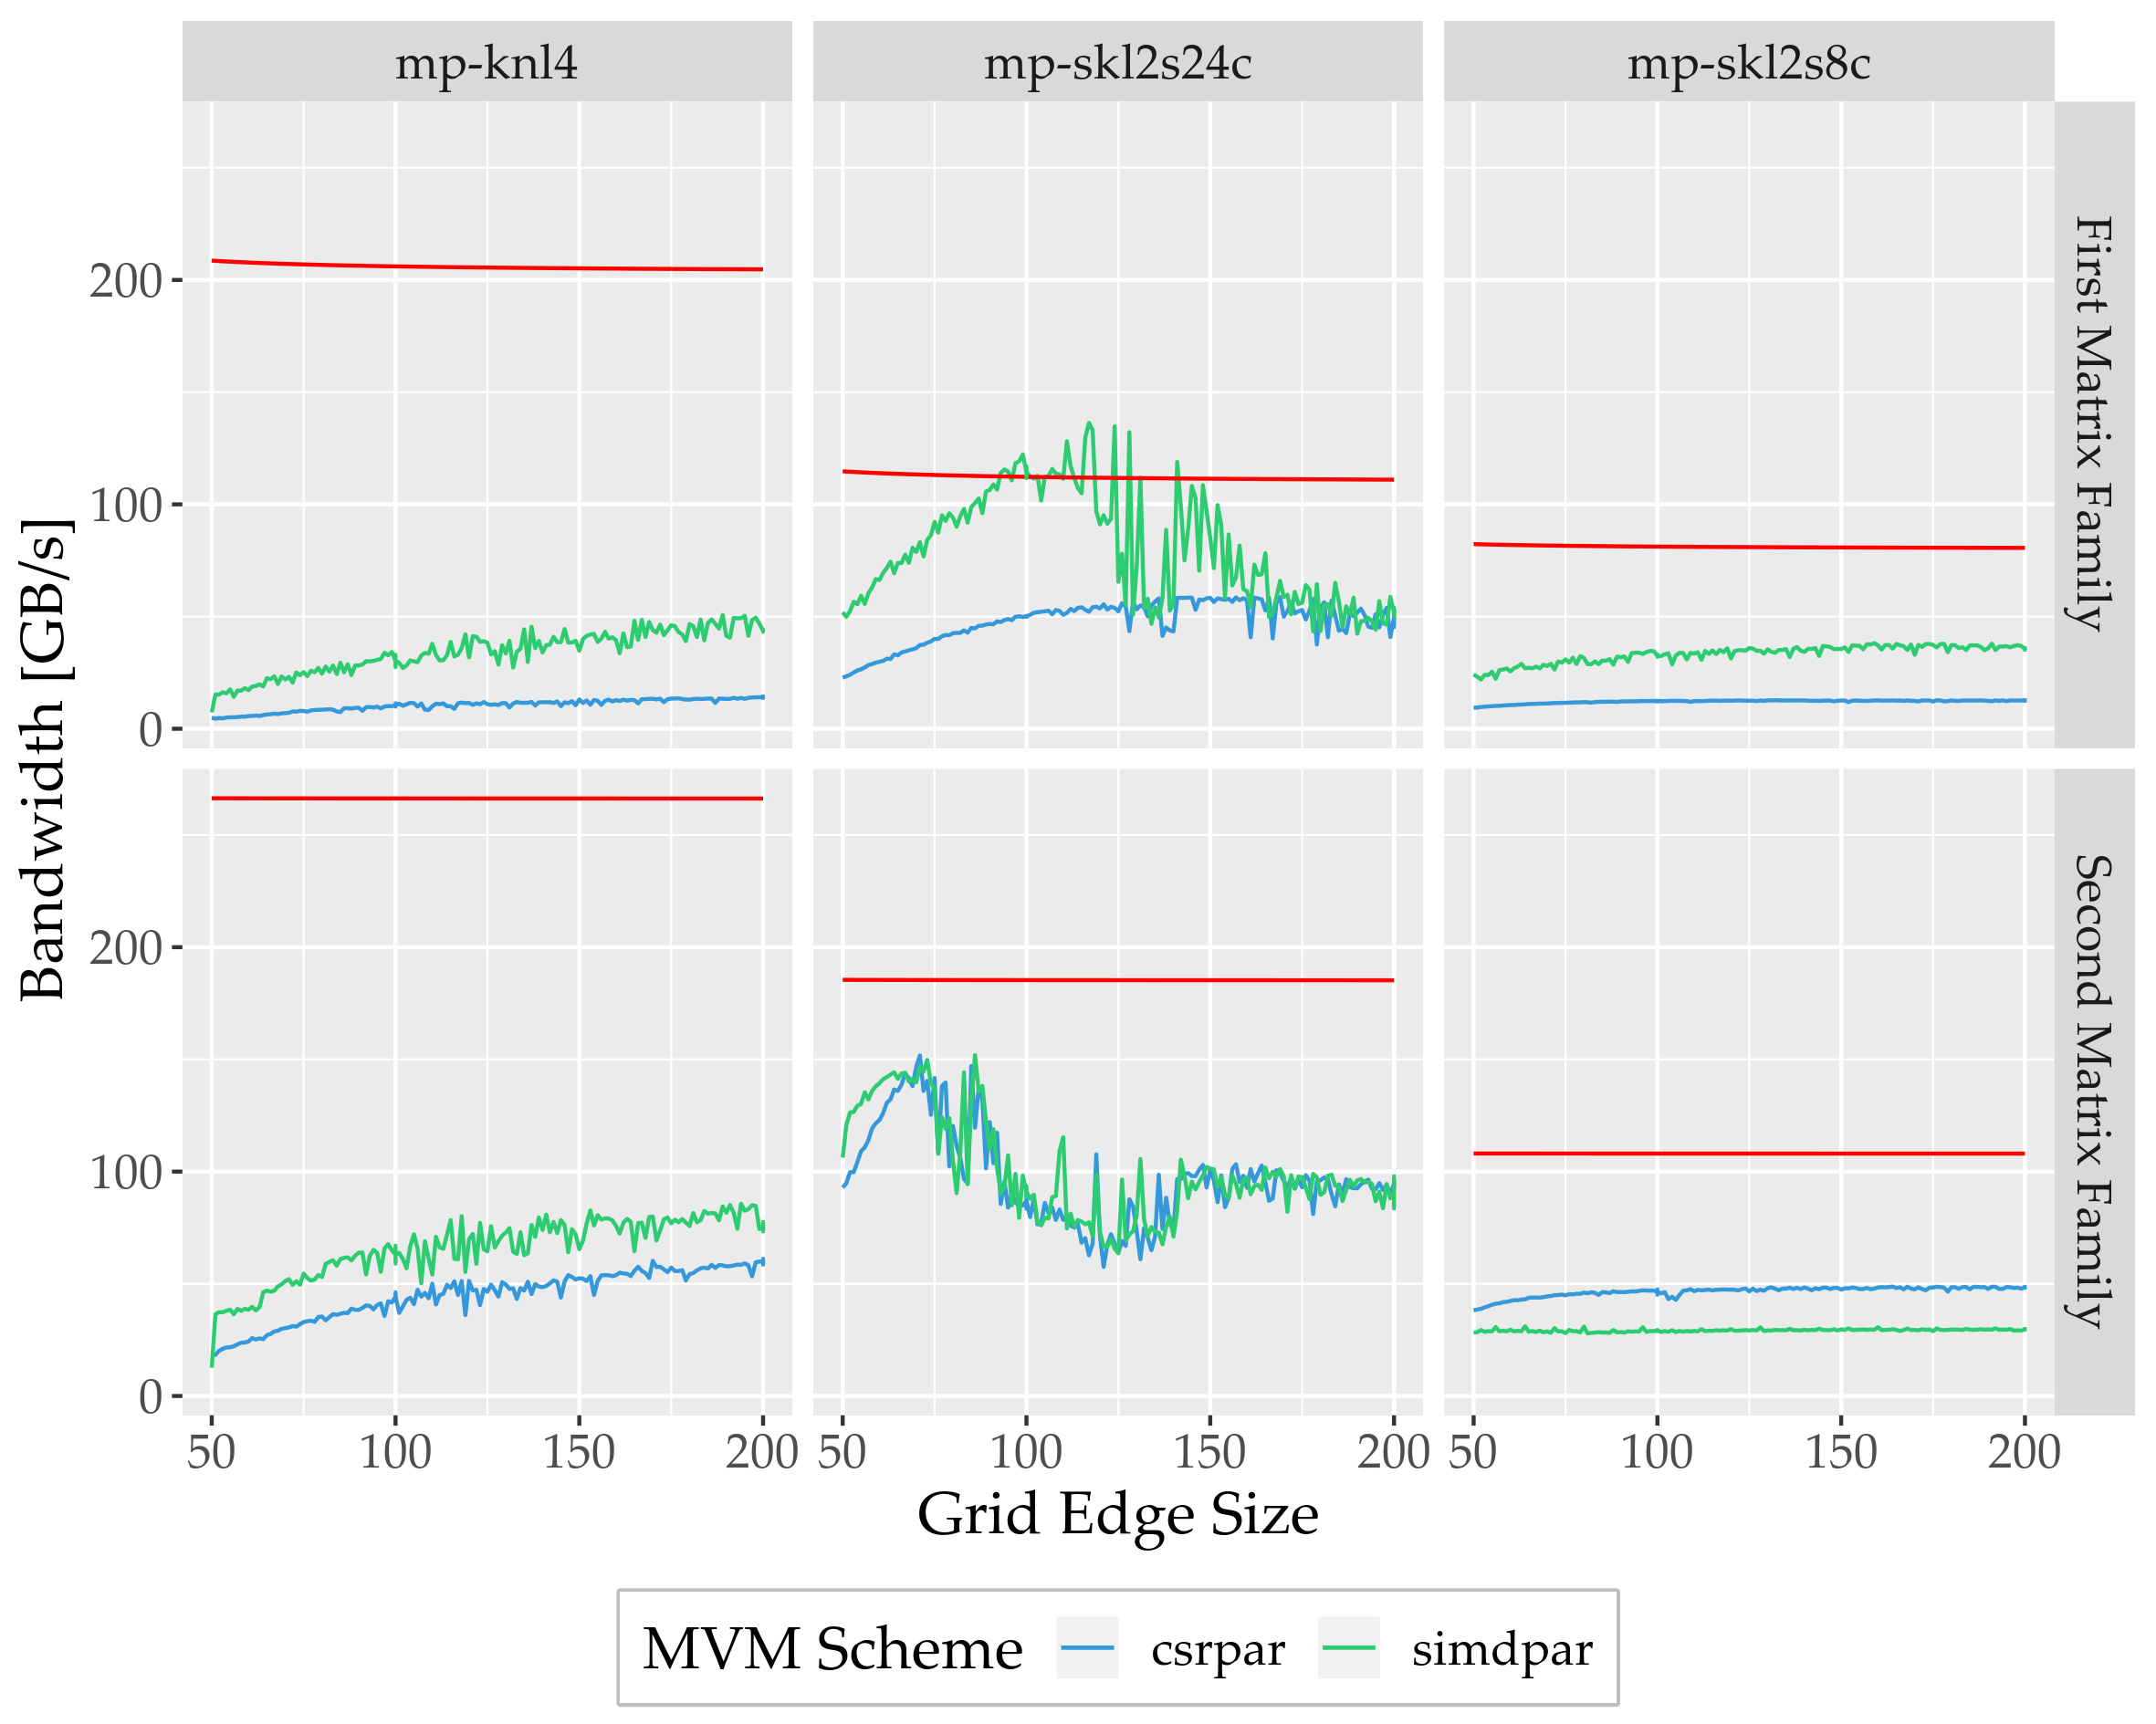
\includegraphics[width=0.9\textwidth]{assets/mvm-perturbed-old}
       \toccaption{todo}{todo}
       \label{fig:mvm-perturbed-old}
     \end{figure}
 
     The plot shows the results for same benchmark as above based on TBB and with a minor difference in implementation,
     which causes the vectorized matrix-vector multiplication to perform badly for second family matrices on the smaller
     Skylake machine. TBB's thread synchronization mechanism is based on a different scheme than the one used by
     Sysmakeshift. The overhead weights significantly less which is demonstrated by the greater performance on the larger
     Skylake and the KNL machines at low to medium grid sizes. Additionally the individual measurements were found to be
     far more dispersed with very large standard deviations which have been omitted from the plot to not render it
     unintelligible.
 
  \section{Matrix-Vector Multiplication of Perturbed Structured Matrices} \label{sec:mvm-perturbed}

    To gauge the stability of the obtained results with respect to disturbances in the matrices' structures the method
    used for the evaluation of the storage density's resilience is applied here again to benchmark the matrix-vector
    multiplication. Perturbations are introduced to a random subset of matrix rows which have their nonzeros' positions
    shuffled and their values randomized. For both families a set of matrices based on a grid with size $d=200$ is
    examined within a range of $0\%$ to $10\%$ perturbed rows. The KNL's values have been omitted due to the
    non-representational results achieved in the benchmark of unperturbed matrices. Figure
    \ref{fig:mvm-perturbed-actually-perturbed} showcases the obtained results. As in the previous benchmark the
    corresponding maximum bandwidth derived from the systems' read and write bandwidths is shown as a gauge of quality.
    Contrasting the above, unperturbed case the bandwidth limits are no longer constant due to the increase in object
    size of the matrix due to the randomization of nonzeros which has been expounded upon in Section
    \ref{sec:objsize-perturbed}. 

    \begin{figure}[H]
      \centering
      \captionsetup{width=0.9\textwidth}
      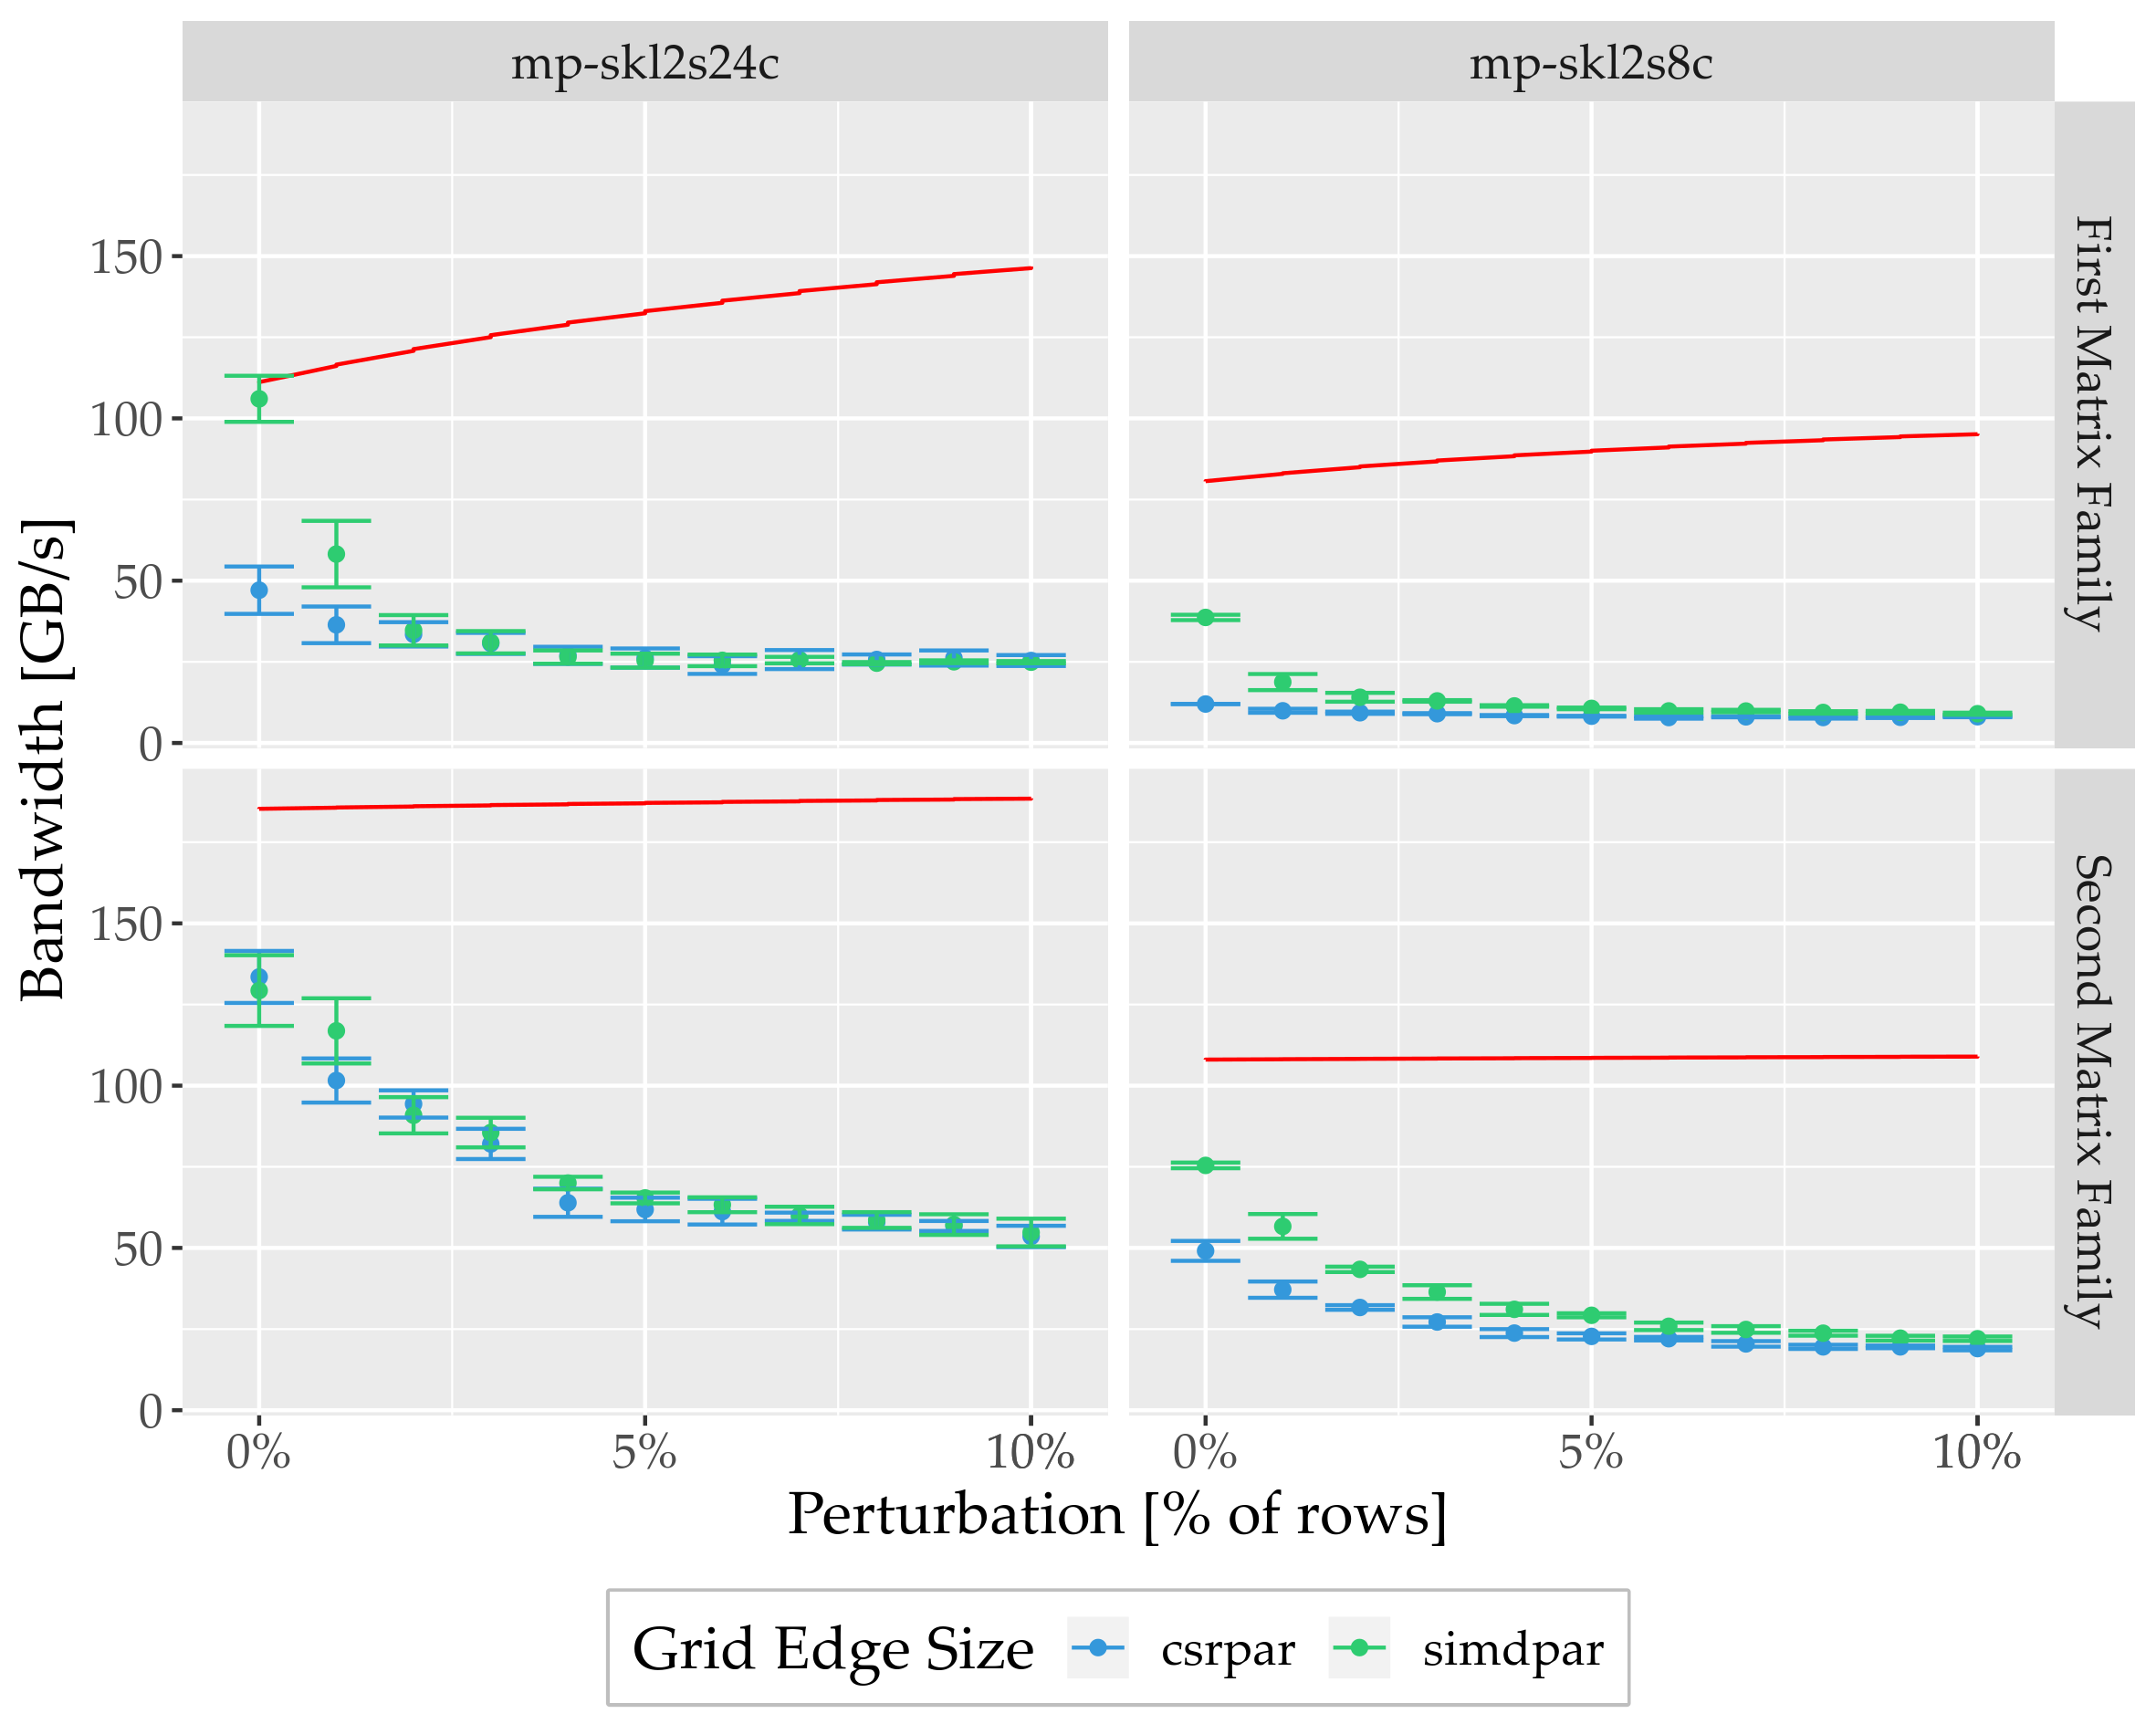
\includegraphics[width=0.9\textwidth]{assets/mvm-perturbed-actually-perturbed}
      \toccaption{todo}{todo}
      \label{fig:mvm-perturbed-actually-perturbed}
    \end{figure}


    In general, the better the performance is for the unperturbed case the more detrimental small perturbations affect
    the obtained bandwidths. Second family matrices show slower declines in bandwidth than their first family
    counterparts. The benchmark displays a convergence of performance of the vectorized multiplication scheme towards
    that of the scalar, CSR-like scheme. This is readily explained by the fact that perturbations introduced into the
    structured matrices disturb the existing matrix segments whose slice compositions are suited for vectorization. This
    causes each of these sets of $8$ contiguous rows to be evaluated via the fallback implementation, which corresponds
    to the CSR-like scheme. Thus, the more rows are perturbed the smaller the percentage of the matrix whose
    matrix-vector multiplication can be performed in a vectorized fashion. As each perturbation disrupts a slice of $8$
    rows even small percentages of total rows perturbed cause both arithmetic schemes to execute virtually the same
    operations producing identical bandwidths as shown in the graphs.

    An important aspect to consider is the fact, that introducing perturbations not only increases disarray in the matrix object's
    data layout but also effectively randomizes accesses into the argument vector $x$. As opposed to fully structured
    matrices which require mostly regular accesses of adjacent or close elements within $x$ a perturbed row entails
    reads of unrelated memory locations at irregular intervals which compromises memory prefetching. Additionally, the
    random accesses elements into $x$ correspond to disparate cache lines which impairs data reusage as
    data, which resides in the cache and which will be required at a later point of execution, is more likely to be
    spuriously evicted. This requires data to be read multiple times raising the effective amount of data movement.

